\documentclass[10pt]{article}
\usepackage{../../local}


\newcommand{\classcode}{Physics 105}
\newcommand{\classname}{Analytic Mechanics}
\renewcommand{\maketitle}{%
\hrule height4pt
\large{Eric Du \hfill \classcode}
\newline
\large{HW 09} \Large{\hfill \classname \hfill} \large{\today}
\hrule height4pt \vskip .7em
\normalsize
}
\linespread{1.1}
\begin{document}
	\maketitle
	\section*{Problem 1}
	A cart of mass $m$ is constrained to move along the $x$-axis. It is attached by a spring (force constant $k$)
	so that the spring is unstretched at $x = 0$. Moreover, a mass $M$ is hangs from the cart by a rigid, 
	massless rod of length $L$. Gravity acts downwards. 

	$$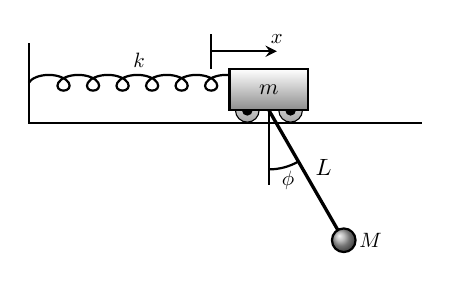
\begin{tikzpicture}
            \draw[thick] (0,1) -- (0,-0.01) -- (5,-0.01);
            \foreach \position in {(2.775,0.15), (3.325,0.15)} {
                \draw[bottom color=gray!70, top color=gray!20!white] \position circle (0.15cm);
                \filldraw[black] \position circle (0.06cm);
            }
            \draw[thick,decoration={aspect=1.6,segment length=3.75mm,amplitude=1mm,coil},decorate] (0,0.5) -- (3,0.5) node[midway,above,yshift=0.1cm,xshift=-0.1cm,scale=0.75] {$k$};
            \draw[thick,bottom color=gray!90,top color=white] (2.55,0.15) -- (2.55,0.675) -- (3.55,0.675) -- (3.55,0.15) -- cycle;
            \node[scale=0.8] at (3.05,0.4125) {$m$};
            \draw[thick] (2.3125,0.675) -- (2.3125,1.125);
            \draw[thick, -stealth] (2.3125,0.9) -- (3.15,0.9) node[above,scale=0.75] {$x$};
            \foreach \position / \thickness / \name in {(3.05,-0.8)/thick/,(4,-1.5)/very thick/L} {
                \draw[\thickness] (3.05,0.15) -- \position node[midway,right,yshift=0.1cm,scale=0.85] {$\name$};
            }
            \shade[ball color=gray!70] (4,-1.5) circle (0.15cm);
            \draw[thick] (4,-1.5) circle (0.15cm) node[right,xshift=0.1cm,scale=0.75] {$M$};
            \draw[thick] (3.05,-0.6) arc (270:300:0.75cm) node[midway,below,yshift=0.05cm,xshift=0.05cm,scale=0.75] {$\phi$};
        \end{tikzpicture}$$
	\begin{enumerate}[label=\alph*)]
		\item Write down the Lagrangian for this system

			\begin{solution}
				The Lagrangian is just the kinetic energy minus potential, so writing out these two terms: 
				\begin{align*}
					T &= \dot x^2(m + M) + \frac{M}{2}\left[ 2 \dot x \dot \phi L \cos \phi + L^2 \dot \phi^2
					\right]\\
					U &= \frac{1}{2}kx^2 + MgL(1 - \cos \phi)
				\end{align*}
				Therefore, the Lagrangian is:
				\[
				\mathcal L = \frac{\dot x^2}{2}(m + M) + \frac{M}{2}\left( 2 \dot x \dot \phi L \cos \phi
				+ L^2 \dot \phi^2 \right) - MgL(1 - \cos \phi) - \frac{1}{2}kx^2
				\] 
			\end{solution}
		\item Simplify your Lagrangian in the case where $x$ and $\phi$ (and derivatives) are small, and derive
			the equations of motion in this approximation

			\begin{solution}
				We use the approximation that $\cos \phi \approx 1 - \frac{\phi^2}{2}$, and also we can 
				get rid of terms which are of order 3 or higher in the coordinates. Therefore, our Lagrangian 
				simplifies to: 
				\[
				\mathcal L = \frac{\dot x^2}{2}(m + M) + \frac{M}{2}\left( 2 \dot x \dot \phi L + L^2 
				\dot \phi^2\right) - MgL(\frac{\phi^2}{2}) - \frac{1}{2}kx^2
				\] 
				Now we find the E-L equations: 
				\begin{align*}
					\pdv{\mathcal L}{x} &= \dv{t} \pdv{\mathcal L}{\dot x} \\
					-kx &= \ddot x(m + M) + ML \ddot \phi \\
					\pdv{\mathcal L}{\phi} &= \dv{t}\pdv{\mathcal L}{\dot \phi} \\
					-MgL\phi &= ML \ddot x + ML^2 \ddot \phi
				\end{align*}
				This implies the equations of motion: 
				\begin{align*}
					-kx &=  \ddot x(m+ M) + ML \ddot \phi \\
					-MgL \phi &= ML \ddot x + ML^2 \ddot \phi 
				\end{align*}
			\end{solution}
		\item Find the normal frequencies.

			\begin{solution}
				Writing this equation in matrix form, this gives us the matrices:
				\[
					\mathbf K = \begin{bmatrix} k & \\ & MgL \end{bmatrix}, \ \ \mathbf M = \begin{bmatrix} m + 
				M & ML \\  ML & ML^2 \end{bmatrix}, \ \mathbf X = \begin{bmatrix} x \\ \phi \end{bmatrix} 
				\] 
				Therefore, so now we need to calculate $\det(\mathbf K - \omega^2\mathbf  M)$:
				\[
				KMgL - 2\omega^2 L^2 k- \omega^2 (m + M) MgL + 2\omega^4(m + M)L^2 - (\omega^2 ML)^2 = 0
				\] 
				This gives solutions: 
				\[
					\omega^2 = \frac{g(m + M) + kL \pm \left[-4gkLm + (-kL - gm - gM)^2\right]^{1/2}}{2Lm}
				\] 
			\end{solution}
		\item Find the normal modes. Sketch the motion of each. You do not have to normalize your modes, and 
			you may write your answers in terms of the corresponding frequencies from the previous part. 

			\begin{solution}
				Since we need only two solutions for $\omega$ to fully describe our system, we can choose 
				the positive root for $\omega$ in the solution above. Further, let $\omega_{\pm}$ refer to 
				these solutions, and $a_1$ and $a_2$ be the components of the eigenvector. Therefore, 
				we are solving the system: 
				\begin{align*}
					ka_1 - \omega_{\pm}^2 (m + M) a_1 - \omega_{\pm}^2 MLa_2 &=  0 \\
					-\omega_{\pm}^2 MLa_1 + MgLa_2 - \omega_{\pm}^2(ML^2)a_2 &= 0
				\end{align*}
				Therefore, from the first equation, we derive $a_2$ in terms of $a_1$:
				\[
					a_2 = \frac{(k - \omega_{\pm}^2(m + M))a_1}{\omega_{\pm}^2 ML}
				\] 
				Then, since $a_1$ and $a_2$ are constants we can write them as $Ae^{i\delta}$, and using the 
				relation between $a_1$ and $a_2$, we get the modes:
				\begin{align*}
					x &= A \cos(\omega_{\pm}t - \delta)\\
					\phi &= \frac{k - \omega_{\pm}^2(m + M)}{\omega^2 Ml}A\cos(\omega t - \delta)
				\end{align*}
				Where $A$ is a constant determined by initial conditions. Furthermore, one of the modes (the positive $\omega_+$) will 
				contribute to the masses oscillating in phase, the other $(\omega_-$) will contribute to them oscillating 
				out of phase. Thanks to Andrew Binder for the Ti\textit kZ diagram:
				$$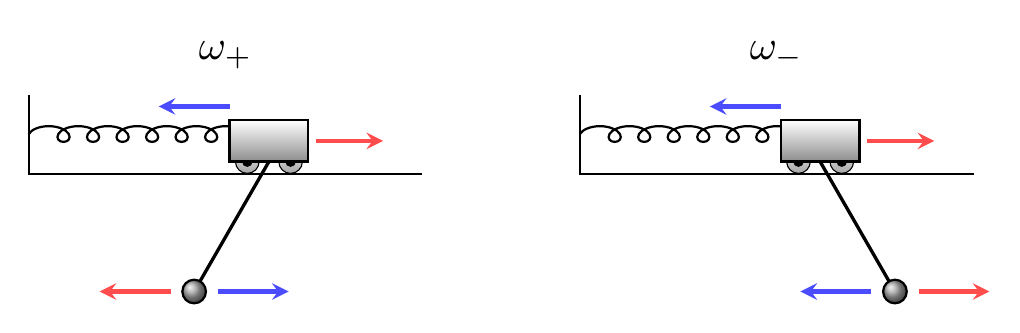
\begin{tikzpicture}
                    \foreach \shift / \frequency / \coord / \icolor / \fcolor in {0/\omega_{+}/2.1/red!70/blue!70,7/\omega_{-}/11/blue!70/red!70} {
                        \draw[thick] (0+\shift,1) -- (0+\shift,-0.01) -- (5+\shift,-0.01);
                        \foreach \position in {(2.775+\shift,0.15), (3.325+\shift,0.15)} {
                            \draw[bottom color=gray!70, top color=gray!20!white] \position circle (0.15cm);
                            \filldraw[black] \position circle (0.06cm);
                        }
                        \node[scale=1.5] at (2.5+\shift,1.5) {$\frequency$};
                        \draw[thick,decoration={aspect=1.6,segment length=3.75mm,amplitude=1mm,coil},decorate] (0+\shift,0.5) -- (3+\shift,0.5);
                        \draw[thick,bottom color=gray!90,top color=white] (2.55+\shift,0.15) -- (2.55+\shift,0.675) -- (3.55+\shift,0.675) -- (3.55+\shift,0.15) -- cycle;
                        \draw[very thick] (3.05+\shift,0.15) -- (\coord,-1.5);
                        \shade[ball color=gray!70] (\coord,-1.5) circle (0.15cm);
                        \draw[thick] (\coord,-1.5) circle (0.15cm);
                        \draw[ultra thick, -stealth, blue!70] (2.55+\shift,0.85) -- (1.65+\shift,0.85);
                        \draw[ultra thick, -stealth, red!70] (3.65+\shift,0.4125) -- (4.5+\shift,0.4125);
                        \draw[ultra thick, -stealth, \icolor] (\coord-0.3,-1.5) -- (\coord-1.2,-1.5);
                        \draw[ultra thick, -stealth, \fcolor] (\coord+0.3,-1.5) -- (\coord+1.2,-1.5);
                    }
                \end{tikzpicture}$$
			\end{solution}
		\item Now suppose there is a small amount of friction acting on the cart, producing a resistive force
			$-b\dot x$. Describe the effect on the normal modes. Is one mode damped? Both?

			\begin{solution}
				We expect both modes to be damped here. The reason is because while the friction only acts on
				the cart, the equations of motion are coupled together, so changes to the acceleration of the 
				cart are also felt by the mass. This occurs in both modes, since there is nothing fundamentally
				different about the masses oscillating in phase or out of phase. 
			\end{solution}
	\end{enumerate}
	\pagebreak
	\section*{Problem 2}

	A thin loop of mass $M$ and radius $R$ oscillates in its own plane. It hangs vertically from a single fixed
	point,
	with gravity acting downwards. Moreover, a bead of the same mass, $M$, is constrained to move (without 
	friction) along the hoop. Find the normal frequencies, normal modes and sketch the motion for each mode. 
	You should find that the eigenfrequencies are: 

	\[
	\omega_1 = \sqrt{\frac{2g}{R}} \ \ \omega_2 = \sqrt{\frac{g}{2R}} 
	\]
	\begin{solution}
		First, we set the point of zero potential to be at the fixed point on the ring. This allows us to 
		express the potential in the easiest way. This potential is equal to: 
		\[
		U = -mgR(\cos \phi_1) - mgR(\cos \phi_1) - mgR(\cos \phi_2)
		\] 
		The kinetic energy of the hoop can be expressed easily as $T_1 = \frac{1}{2}I \dot \phi_1^2$, but the 
		kinetic energy of the bead is slightly trickier. We can make it slightly easier by writing it out in 
		cartesian coordinates, from which we can get:
		\[
		x = R \sin \phi_1 + R \sin \phi_2\ \ y = -R \cos \phi_1 - R \cos \phi_2
		\] 
		Therefore, the kinetic energy is (skipping some algebra)
		\[
		T = \frac{m}{2}(R^2(\dot \phi_1 \cos \phi_1 + \dot \phi_2 \cos \phi_2)^2 + R^2(\dot \phi_1 \sin \phi_1 + 
		\dot \phi_2 \sin \phi_2)^2) = \frac{mR^2}{2}\left[\dot \phi_1^2 + \dot \phi_2^2 + 2 \dot \phi_1 \dot 
		\phi_2 \cos(\phi_1 - \phi_2)\right] 
		\] 
		So the Lagrangian is: 
		\[
		\mathcal L = \frac{1}{2}I\dot \phi_1^2 + \frac{MR^2}{2}\left[\dot \phi_1^2 + \dot \phi_2^2 + 2\dot \phi_1
		\dot \phi_2 \cos(\phi_1 - \phi_2)\right] + mgR(2 \cos \phi_1 + \cos \phi_2)
		\] 
		Using the small angle approximation of $\cos \theta \approx 1 - \frac{\theta^2}{2}$, we now get: 
		\[
		\mathcal L = \frac{1}{2}I \dot \phi_1^2  + \frac{MR^2}{2}(\dot \phi_1 + \dot \phi_2)^2 + 2MgR(1 - 
		\frac{\phi_1^2}{2})
		\] 
		Then, computing Euler-Lagrange equations, we get the following system: 
		\begin{align*}
			-2MgR\phi_1 &= 3MR^2\ddot \phi_1 + MR^2 \ddot \phi_2 \\
			-MgR\phi_2 &= MR^2 \ddot \phi_1 + MR^2 \ddot \phi_2
		\end{align*}

		Therefore, our matrices are:
		\[
			\mathbf K = MgR\begin{bmatrix} 2 & \\ & 1 \end{bmatrix} , \ \mathbf M = MR^2\begin{bmatrix} 3 & 1
		\\ 1 & 1\end{bmatrix}, \ \mathbf x = \begin{bmatrix} \phi_1\\ \phi_2 \end{bmatrix} 
		\] 
		Now, the determinant of this system is: 
		\[
		\det(\mathbf K - \omega^2 \mathbf M) = 2M^2g^2R^2 - \omega^2 MgR + 2M\omega^4 = 0
		\] 
		This gives the solutions: 
		\[
		\omega^2 = \frac{g}{2R}, \frac{2g}{R} \implies \omega_1 = \sqrt{\frac{g}{2R}}, \omega_2 =
		\sqrt{\frac{2g}{R}} 
		\] 
		as expected from the problem statement. The corresponding eigenvectors are:
		\[
		\mathbf a = \begin{bmatrix} a_1\\ a_2 \end{bmatrix} = \begin{bmatrix} 1\\ 1 \end{bmatrix} ,
		\begin{bmatrix} -\frac{1}{2} \\1  \end{bmatrix} 
		\] 
		For the $a_1 = a_2 = 1$, the oscillations are: 
		\begin{align*}
			\phi_1(t) &= A\cos\left(\sqrt{\frac{g}{2R}} - \delta\right) \\
			\phi_2(t) &= A \cos\left(\sqrt{\frac{g}{2R}}t - \delta\right) \\
		\end{align*}
		In other words, they oscillate in phase with one another. In the other mode, the oscillations are: 
		\begin{align*}
			\phi_1(t) =\frac{1}{2} A\cos\left( \sqrt{\frac{2g}{R}}t - \delta \right) \\
			\phi_2(t) =	-A \cos\left( \sqrt{\frac{2g}{R}}t - \delta \right)  
		\end{align*}
		Here, the oscillations are out of phase with one another, and further the bead oscillates with 
		an amplitude which is twice that of the hoop. Here's a diagram: 
		$$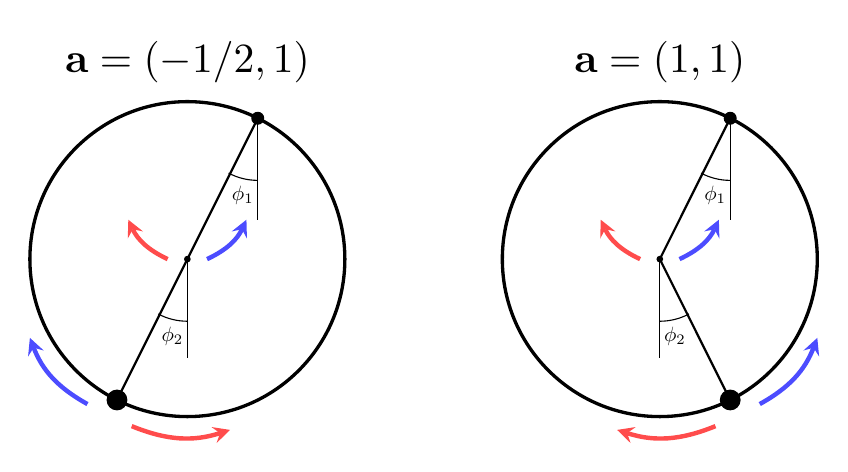
\begin{tikzpicture}
            \foreach \shift / \position / \angle / \istart / \iend / \fstart / \fend / \bend in {0/-0.894/-28/-1.269/-1.841/-2/-1/left,6/6.894/28/7.269/-1.841/8/-1/right} {
                \filldraw[black] (\shift,0) circle (0.035cm);
                \draw[very thick] (\shift,0) circle (2cm);
                \filldraw[black] (0.894+\shift,1.789) circle (0.075cm);
                \draw[thick] (\shift,0) -- (0.894+\shift, 1.789);
                \draw[thin] (0.894+\shift,1.789) -- (0.894+\shift,0.5);
                \draw (0.894+\shift,1) arc (270:242:0.789cm) node[midway,below,scale=0.75] {$\phi_1$};
                \draw[thin] (\shift,0) -- (\shift,-1.25);
                \filldraw[black] (\position,-1.789) circle (0.125cm);
                \draw[thick] (\shift,0) -- (\position,-1.789);
                \draw (\shift,-0.789) arc (270:270+\angle:0.789cm) node[midway,below,scale=0.75] {$\phi_2$};
                \draw[ultra thick, -stealth, red!70] (-0.25+\shift,0) to[bend left=20] (-0.75+\shift,0.5);
                \draw[ultra thick, -stealth, blue!70] (0.25+\shift,0) to[bend right=20] (0.75+\shift,0.5);
                \draw[ultra thick, -stealth, blue!70] (\istart,\iend) to[bend \bend=20] (\fstart,\fend);
            }
            \draw[ultra thick, -stealth, red!70] (-0.707,-2.121) to[bend right=20] (0.542,-2.169);
            \draw[ultra thick, -stealth, red!70] (6.707,-2.121) to[bend left=20] (5.458,-2.169);
            \node[scale=1.5] at (0,2.5) {$\mathbf a = (-1/2, 1)$};
            \node[scale=1.5] at (6,2.5) {$\mathbf a = (1, 1)$};
        \end{tikzpicture}$$
		In the left figure, we can see that the masses oscillate out of phase with respect to one another, and specifically the second mass oscillates with an amplitude twice that of the hoop. This corresponds to the eigenvector $\mathbf a = (-1/2, 1)$. In the other case, we see that the masses oscillate in phase relative to one another, with the same amplitude of oscillation, corresponding to the eigenvector $\mathbf a = (1, 1)$
	\end{solution}
	


	\pagebreak

	\section*{Problem 3}
	Three particles of equal mass $m$ move on a circle with radius $a$ under forces that can be derived 
	from the potential
	\[
		V(\alpha, \beta, \gamma) = V_0\left( e^{-2\alpha} + e^{-2\beta} + e^{-2\gamma} \right) 
	\] 
	where $\alpha, \beta, \gamma$ are the angular separations of the masses (in radians) as shown in the figure
	below. An equilibrium position is indicated by the solid lines extending beyond the circle and has $\alpha = 
	\beta = \gamma = 2\pi/3$. In the following parts, $\theta_i$ represents the deviation from this equilibrium
	of the $i$th mass in the clockwise direction (see figure)

	$$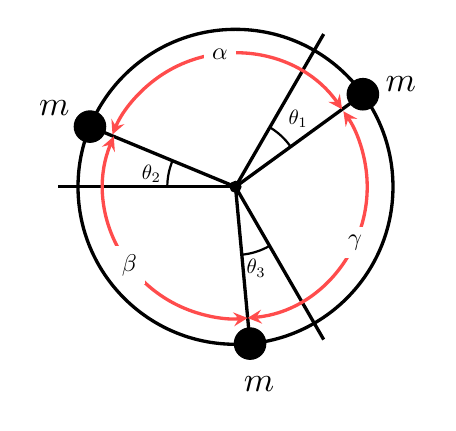
\begin{tikzpicture}
            \draw[very thick] (0,0) circle (2cm);
            \filldraw[black] (0,0) circle (0.07cm);
            \foreach \position in {(1.618,1.176), (-1.848,0.765), (.185,-1.991)} {
                \filldraw[black] \position circle (0.2cm);
                \draw[very thick] (0,0) -- \position;
            }
            \foreach \position in {(2.1,1.3), (-2.3,1), (0.3,-2.5)} {
                \node[scale=1.25] at \position {$m$};
            }
            \foreach \position in {(1.12,1.94), (-2.25,0), (1.12,-1.94)} {
                \draw[very thick] (0,0) -- \position;
            }
            \foreach \position / \start / \end / \label in {(1.354,0.984)/35/157.5/\alpha, (-1.546,0.64)/157.5/275.29/\beta, (0.154,-1.666)/275.29/395/\gamma} {
                \draw[very thick, red!70,stealth-stealth] \position arc (\start:\end:1.673cm) node[midway,black,fill=white,scale=0.875] {$\label$};
            }
            \foreach \position / \start / \end / \label / \location in {(0.701,0.509)/35/60/\theta_1/above right, (-0.8,0.331)/157.5/180/\theta_2/left, (0.08,-0.862)/275.29/300/\theta_3/below} {
                \draw[thick] \position arc (\start:\end:0.866cm) node[midway,\location,black,scale=0.75] {$\label$};
            }
        \end{tikzpicture}$$
	\begin{enumerate}[label=\alph*)]
		\item Find the normal mode frequencies using the small amplitude approximation for oscillations about 
			equilibrium. 

			\begin{solution}
				The Lagrangian is: 
				\[
				\mathcal L = \frac{ma^2}{2}(\dot \theta_1^2 + \dot \theta_2^2 + \dot \theta_3^2) - 
				V_0e^{-4\pi/3}\left[e^{-2(\theta_1 - \theta_2)} + e^{-2(\theta_2 - \theta_3)} + e^{-2(\theta_3
				- \theta_1)}\right]
				\] 
				Therefore, the equations of motion from doing the Euler-Lagrange equations becomes: 
				\begin{align*}
					ma^2 \ddot \theta_1  &= -2V_0e^{-4\pi/3}\left[e^{-2(\theta_3 - \theta_1)} -
					e^{-2(\theta_1 - \theta_2)}\right] \\
					ma^2 \ddot \theta_2 &= -2V_0e^{-4\pi/3}\left[e^{-2(\theta_1 - \theta_2)} -
					e^{-2(\theta_2 - \theta_3)}\right] \\
					ma^2 \ddot \theta_3 &= -2V_0e^{-4\pi/3} \left[e^{-2(\theta_2 - \theta_3)} - 
					e^{-2(\theta_3 - \theta_1)}\right]
				\end{align*}
				Then, using the approximation for small amplitude, we write $e^x \approx 1 + x$, which simplifies
				our equations to: 
				\begin{align*}
					ma^2 \ddot \theta_1 &= -2V_0e{-4\pi/3}(4\theta_1 - 2\theta_2 - 2\theta_3)\\
					ma^2 \ddot \theta_2 &= -2V_0e^{-4\pi/3}(4 \theta_2 - 2\theta_1 - 2\theta_3)\\
					ma^2 \ddot \theta_3 &= -2V_0e^{-4\pi/3}(4\theta_3 - 2\theta_1 - 2\theta_2)
				\end{align*}
				This means that our matrices are: 
				\[
					\mathbf M = ma^2\begin{bmatrix} 1 & &\\ & 1 & \\ & & 1 \end{bmatrix} = ma^2I, \ 
					\mathbf K = 4V_0e^{-4\pi/3}\begin{bmatrix} 2 & -1 & -1\\-1&2&-1\\-1&-1&2 \end{bmatrix} , \ \
					\mathbf X = \begin{bmatrix} \theta_1 \\ \theta_2 \\ \theta_3 \end{bmatrix} 
				\] 
				Solving this system gives: 
				\[
					\omega_1^2 =0, \omega_{2, 3}^2 = \frac{12e^{-4\pi/3}V_0}{a^2m}
				\]
			\end{solution}
		\item Find the corresponding normal modes. 

			\begin{solution}
				Solving the eigenvectors from the solution in part (a) gives: 				
				\[
				a = (1, 1, 1), (-1, 0, 1), (1, -1, 0)
				\] 
				Here, there are three modes to this system, which give the equations: 
				\begin{align*}
					\theta_1(t) &= (V_0t + \theta_0)\begin{pmatrix} 1\\1\\1 \end{pmatrix}  \\
					\theta_2(t) &= \begin{pmatrix} -1\\0\\1 \end{pmatrix} A \cos(\omega_2 t - \delta)\\
					\theta_3(t) &= \begin{pmatrix} 1 \\ -1 \\ 0 \end{pmatrix} A \cos(\omega_3t - \delta)
				\end{align*}
				Where the index on the left hand side refers to the mode of oscillation. 


				These normal modes make complete sense: in one of the modes, all the masses are shifted by the
				same angle $\theta$, so it makes sense that no oscillatory motion occurs there. In the other 
				two cases, we see that two masses oscillate such that they move out of phase with respect
				to each other, while the third mass remains stationary. The third mode is the same thing, 
				except we have a different mass remaining stationary. 
			\end{solution}
		\item Sketch the motion for each of the normal modes you found in (b)


			\begin{solution}
				I've described the oscillation in the previous part, here's the diagram (credit to Andrew Binder for the visualization)

				$$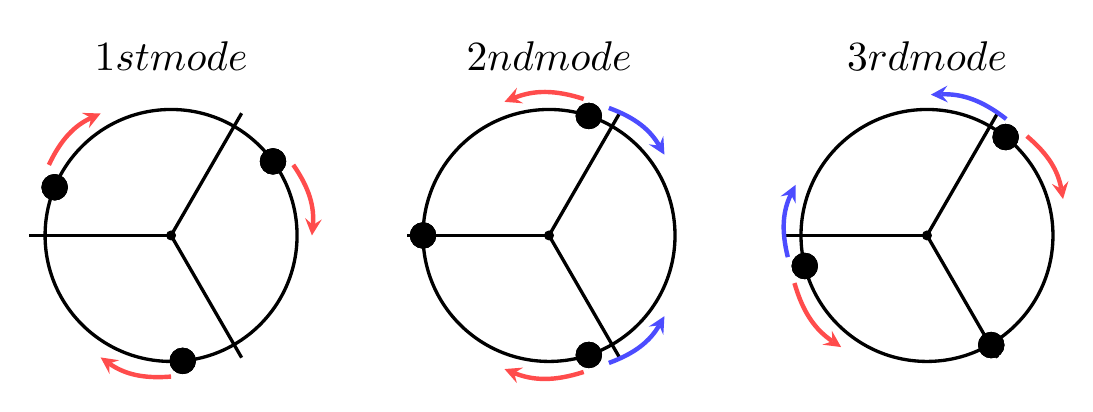
\begin{tikzpicture}[scale=0.8]
                    \foreach \shift / \mode in {0/\text{1st mode}, 6/\text{2nd mode}, 12/\text{3rd mode}} {
                        \draw[very thick] (0+\shift,0) circle (2cm);
                        \filldraw[black] (0+\shift,0) circle (0.07cm);
                        \foreach \position in {(1.618,1.176), (-1.848,0.765), (0.185,-1.991), (4,0), (13.249,1.562), (10.06,-0.485), (6.632,1.897), (13.02,-1.74), (6.632,-1.897)} {
                            \filldraw[black] \position circle (0.2cm);
                        }
                        \foreach \position in {(1.12+\shift,1.94), (-2.25+\shift,0), (1.12+\shift,-1.94)} {
                            \draw[very thick] (0+\shift,0) -- \position;
                        }
                        \node[scale=1.5] at (\shift, 2.85) {$\mode$};
                    }
                    \foreach \angle in {-30,90,210} {
                        \draw[ultra thick, -stealth, red!70, rotate=\angle] (1.12,-1.94) to[bend left=20] (0,-2.236);
                    }
                    \draw[ultra thick, -stealth, red!70] (6.55,2.167) to[bend right=20] (5.293,2.121);
                    \draw[ultra thick, -stealth, blue!70] (6.95,2.024) to[bend left=20] (7.832,1.282);
                    \draw[ultra thick, -stealth, red!70] (6.55,-2.167) to[bend left=20] (5.293,-2.121);
                    \draw[ultra thick, -stealth, blue!70] (6.95,-2.024) to[bend right=20] (7.832,-1.282);
                    \draw[ultra thick, -stealth, blue!70,rotate around={-20:(12,0)}] (12.55,2.167) to[bend right=20] (11.293,2.121);
                    \draw[ultra thick, -stealth, red!70,rotate around={-20:(12,0)}] (12.95,2.024) to[bend left=20] (13.832,1.282);
                    \draw[ultra thick, -stealth, red!70,rotate around={124:(12,0)}] (12.55,2.167) to[bend right=20] (11.293,2.121);
                    \draw[ultra thick, -stealth, blue!70,rotate around={124:(12,0)}] (12.95,2.024) to[bend left=20] (13.832,1.282);
                \end{tikzpicture}$$
				Here, we can see that the first mode corresponds to all the masses moving together, where $\omega = 0$. In the other two cases, we have one mass stationary, while the other two masses oscillate. They are ``in phase'' in the sense that they both move toward and away from the stationary mass at the same time. Mathematically though, they are expressed as being out of phase. 
			\end{solution}
		\item Consider the following initial conditions at $t = 0$: $\theta_1 = \theta_2 = \theta_3 = 0$, 
			$\dot \theta_1 = 3\omega_0$, $\dot \theta_2 = -2\omega_0$, and $\dot \theta_3 = -\omega_0$. If 
			$\omega_0$ is sufficiently small, then the small amplitude approximation will be valid. In this case,
			use your results above to find $\theta_i(t)$ for $i = 1, 2, 3$. 

			\begin{solution}
				Since the initial conditions are $\theta_1 = \theta_2 = \theta_3 = 0$, so we expect our 
				oscillatory solutions to be sinusoids. Further, our amplitudes are the initial velocities 
				divided by $\omega_0$. Therefore, the equations of motion are: 
				\begin{align*}
					\theta_1(t) &=  \frac{3\omega_0}{\omega}\sin(\omega t) \\
					\theta_2(t) &=  -\frac{2\omega_0}{\omega}\sin (\omega t) \\
					\theta_3(t) &= -\frac{\omega_0}{\omega}\sin (\omega t)
				\end{align*}
			\end{solution}

		\item Now suppose instead $\dot \theta_1 = 4\omega_0$, $\dot \theta_2 = -\omega_0$ and $\dot \theta_3 
			= 0$ (we have added $\omega_0$ to each angular velocity). What are the new functions for 
			$\theta_i(t)$? You should be able to answer this part without any new computations. 
			
			\begin{solution}
				The oscillation will be exactly what we expect: the same normal modes, but this time with 
				an added term which describes the addition of velocity: 
				\[
				\theta_i'(t) = \theta_i(t) + \omega_0t
				\] 
			\end{solution}
		\item How small should $\omega_0$ be for (d) to hold? Write your answer in the form $\omega_0 \ll$ 
			something. 
		
			\begin{solution}
				In order for our approximations to hold, we require that $\omega_0 \ll \omega$, since otherwise
				the initial velocities would dominate over the oscillatory ones. 
			\end{solution}
	\end{enumerate}

	\pagebreak
	\section*{Python Homework}
	The double pendulum is pictured below:

	[inset tikz here]
	\begin{enumerate}[label=\alph*)]
		\item Show that the Lagrangian of the system is given by 
		\begin{multline*}
		\mathcal L = \frac{1}{2}(m_1 + m_2)L_1^2 \dot \phi_1^2 + \frac{1}{2}m_2 L_2^2 \phi_2^2 +
		m_2L_1L_2 \dot \phi_1 \dot \phi_2 \cos(\phi_2 - \phi_1) -\\ (m_1 + m_2)gL_1(1-\cos \phi_1) -
		m_2gL_2(1 - \cos \phi_2)
		\end{multline*}

		\begin{solution}
			Let the potential energy be measured relative to the configuration in which both masses are hanging
			straight down. Then, we can write the potential energy as:
			\[
			U = m_1gL_1(1 - \cos \phi_1) + m_2gL_1(1 - \cos \phi_1) + m_2gL_2(1 - \cos \phi_2) 
			\] 
			To calculate the kinetic energy term, we express the coordinates of the second mass in the following
			way: 
			\begin{align*}
				X &= L_1 \sin \phi_1 + L_2 \sin \phi_2\\
				Y &= -L_1 \cos \phi_1 - L_2 \cos \phi_2
			\end{align*}
			And since the kinetic energy is $\frac{1}{2}m_2(\dot X^2 + \dot Y^2)$, we get: 
			\begin{align*}
				T_2 &= \frac{1}{2}m_2\left[L_1^2 \dot \phi_1^2 + L_2^2 \dot \phi_2^2 + 2L_1L_2\dot \phi_1
				\dot \phi_2 (\cos \phi_1 \cos \phi_2 + \sin \phi_1 \sin \phi_2)\right]\\
					&= \frac{1}{2}m_2\left[L_1^2 \dot \phi_1^2  + L_2^2 \dot \phi_2^2 + 2L_1L_2\cos(\phi_2 -
					\phi_1)\right]  \\
			\end{align*}
			Combining this with the kinetic energy term for the first mass, we have: 
			\[
			T = \frac{1}{2}m_1L_1^2 \dot \phi_1^2 + \frac{1}{2}m_2\left[ L_1^2 \dot \phi_1^2 + 
			L_2^2 \dot \phi_2^2 + 2L_1L_2 \cos(\phi_2 - \phi_1)\right]
			\] 
			Therefore, the Lagrangian is (with a little bit of rearrangement): 
			\begin{multline*}
			\mathcal L = \frac{1}{2}(m_1 + m_2)L_1^2 \dot \phi_1^2 + \frac{1}{2}m_2 L_2^2 \dot \phi_2^2 + 
			m_2L_1L_2 \dot \phi_1 \dot \phi_2 \cos(\phi_2 - \phi_1) -\\ (m_1 + m_2)gL_1(1-\cos \phi_1) -
			m_2gL_2(1 - \cos \phi_2)
			\end{multline*} 
			as desired. 
		\end{solution}
	\item Find the equations of motion

		\begin{solution}
			We have the Lagrangian, so we just have to use the Euler-Lagrange equations. There are two 
			coordinates $\phi_1$ and $\phi_2$, so first for $\phi_1$: 
			\[
				\pdv{\mathcal L}{\phi_1} = \dv{t}\pdv{\mathcal L}{\dot \phi_1}\\
			\]			
			This gets the equation: 
			\begin{multline*}
				m_2L_1L_2 \dot \phi_1 \dot \phi_2 \sin(\phi_2 - \phi_1) - (m_1 + m_2)gL_1 \sin \phi_1 \\=
										  (m_1 + m_2)L_1^2 \ddot \phi_1 +\ m_2L_1L_2 \left[\ddot \phi_2 \cos(\phi_2 - \phi_1) -\dot \phi_2
				\sin(\phi_2 - \phi_1)(\dot \phi_2 - \dot \phi_1)\right]
			\end{multline*}
			Similarly, the equation for $\phi_2$ gets: 
			\begin{multline*}
				-m_2L_1L_2 \dot \phi_1 \dot \phi_2 \sin(\phi_2 - \phi_1) - m_2gL_2\sin \phi_2\\
				= m_2L_2^2\ddot \phi_2 + m_2L_1L_2\left[\ddot \phi_1 \cos(\phi_2 - \phi_1) - \dot \phi_1
				\sin (\phi_2 - \phi_1)(\dot \phi_2 - \dot \phi_1)\right]
			\end{multline*}
		\end{solution}
	\item Under the small angle approximation $\phi_1, \phi_2 \ll 1$ (keeping only first-order terms), find the
		normal modes of oscillation, which is pictured below for a simple choice of parameters.

		\begin{solution}
			So if we keep only the first order terms, then we use the approximations $\sin \theta \approx \theta$
			and $\cos \theta \approx 1$. If we do this, the cross term with $(\dot \phi_2 - \dot \phi_1)$ term
			dies because it's of a higher order. Therefore, we get the equations: 
			\begin{align*}
				-(m_1 + m_2)gL_1 \sin \phi_1 &= (m_1 + m_2) L_1^2 \ddot \phi_1 + m_2L_1L_2 \ddot \phi_2\\
				-m_2gL_2 \sin \phi_2 &= m_2L_2^2 \ddot \phi_2 + m_2L_1L_2\ddot \phi_1
			\end{align*}
			Therefore, our matrices are: 
			\[
				\mathbf K = \begin{bmatrix} (m_1 + m_2)gL_1 & \\ & m_2gL_2 \end{bmatrix}, \ \  
				\mathbf M = \begin{bmatrix} (m_1 + m_2)L_1^2 & m_2L_1L_2\\ m_2L_1L_2 & m_2L_2^2 \end{bmatrix},
				\ \ \mathbf x = \begin{bmatrix} \phi_1 \\ \phi_2 \end{bmatrix} 
			\]
			Therefore, solving $\det(\mathbf K - \omega^2 \mathbf M) = 0$ means to find solutions to $\omega$ 
			that satisfy: 
			\[
				m_2L_1L_2g^2\left[(m_1 + m_2)g^2 - g(L_1 + L_2)(m_1 + m_2)\omega^2 + L_1L_2m_1 \omega^4\right]=0
			\] 
			This then gives solutions (using WolframAlpha): 
			\[
				\omega_{1, 2}^2 = \frac{g(L_1 + L_2)(m_1 + m_2) \pm \left[g^2(L_1 + L_2)^2(m_1 +m_2)^2 - 4g^2L_1
				L_2m_1(m_1 + m_2)\right]^{1/2}}{2m_1L_1L_2}
			\] 
			Again just like problem 1, we will only take positive solutions to this equation since there are
			only two normal modes. To find the components to the eigenvectors, we express $a_1$ in terms of 
			$a_2$, which we can do from the equation: 
			\[
				-\omega_{1, 2}^2 m_2L_1L_2a_1 + \left[m_2gL_2 - \omega_{1, 2}m_2L_2^2\right]a_2 = 0
			\] 
			This means that: 
			\[
				a_1 = \frac{(m_2gL_2 - \omega_{1, 2}^2 m_2L_2^2)a_2}{\omega_{1, 2}m_2L_1L_2}
			\] 
			This means that the oscillation modes are:
			\begin{align*}
				\phi_1(t) &= \frac{(m_2gL_2 - \omega_{1, 2}^2 m_2L_2^2)}{\omega_{1, 2}m_2L_1L_2}A 
				\cos(\omega_{1, 2} + \delta)\\
				\phi_2(t) &= A \cos(\omega_{1, 2} + \delta)
			\end{align*}
			Where $A$ is a constant that is determined via initial conditions. 
		\end{solution}

	\end{enumerate} 
\end{document}
